\section{\textit{Embeddings}}

gesnim word2vec model

Parameters:
\begin{itemize}
    \item Embedding Size:
    
    \item Window:
    
    \item Min Count:
    
    \item SG:
    
    \item Negative:
\end{itemize}

\subsection{2D Plots}

PCA

\subsubsection{Simpsons Dataset}

\begin{figure}[H]

\centering
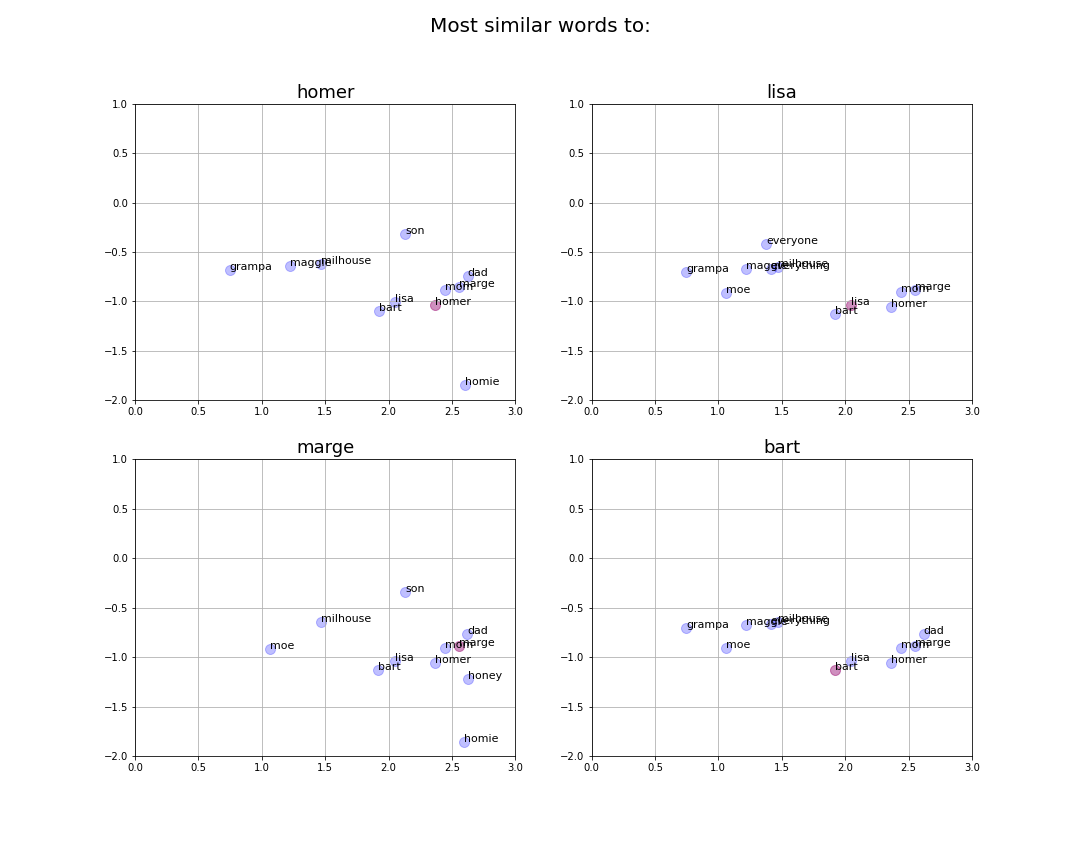
\includegraphics[width=.3\textwidth]{results/embeddings/simpsons_similar_15.png}\hfill
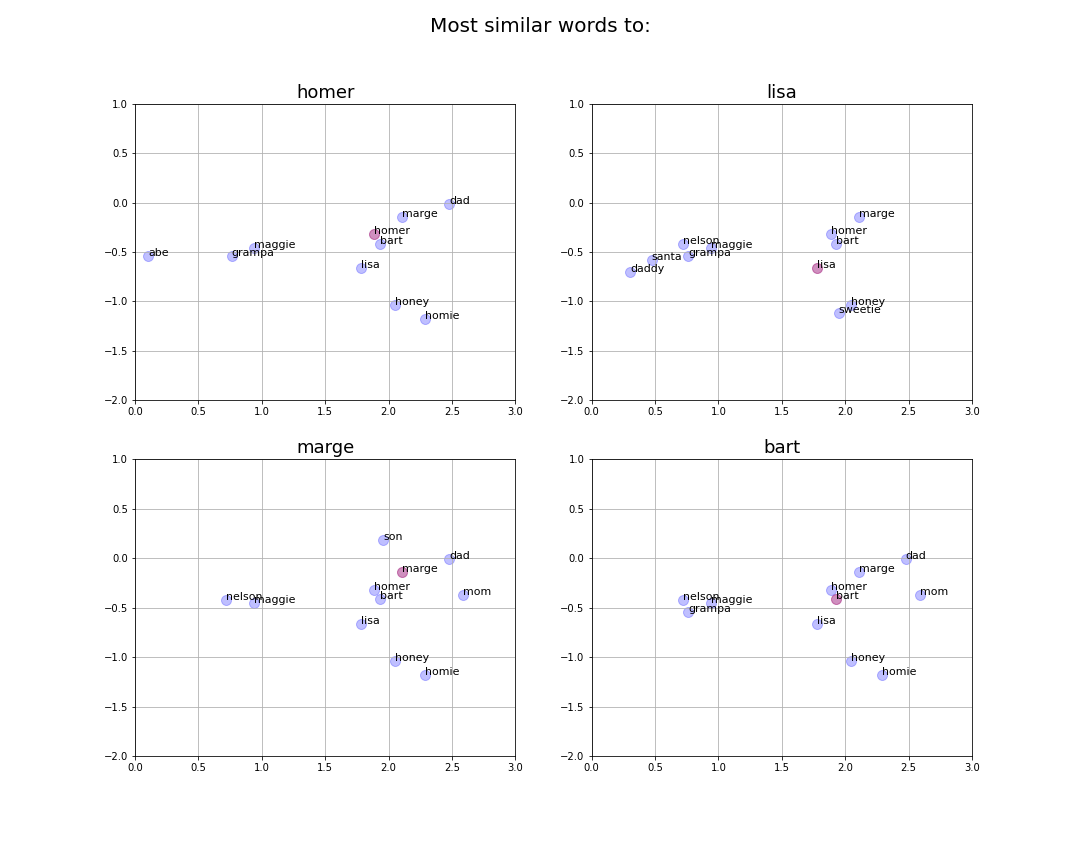
\includegraphics[width=.3\textwidth]{results/embeddings/simpsons_similar_75.png}\hfill
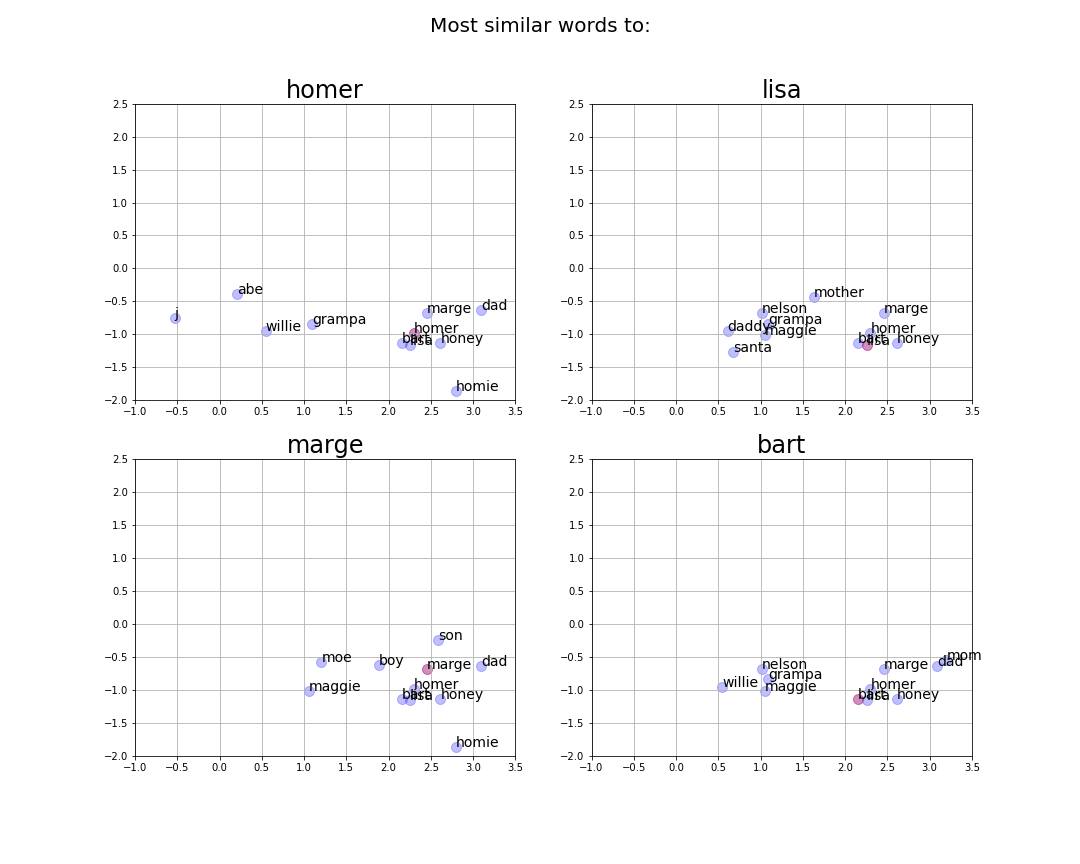
\includegraphics[width=.3\textwidth]{results/embeddings/simpsons_similar_150.png}
\caption{Simpsons main character in 2D plot with similar words for different embeddings size}
\label{fig:simpsons_sim_words}

\end{figure}


\subsubsection{Friends Dataset}

\begin{figure}[H]

\centering
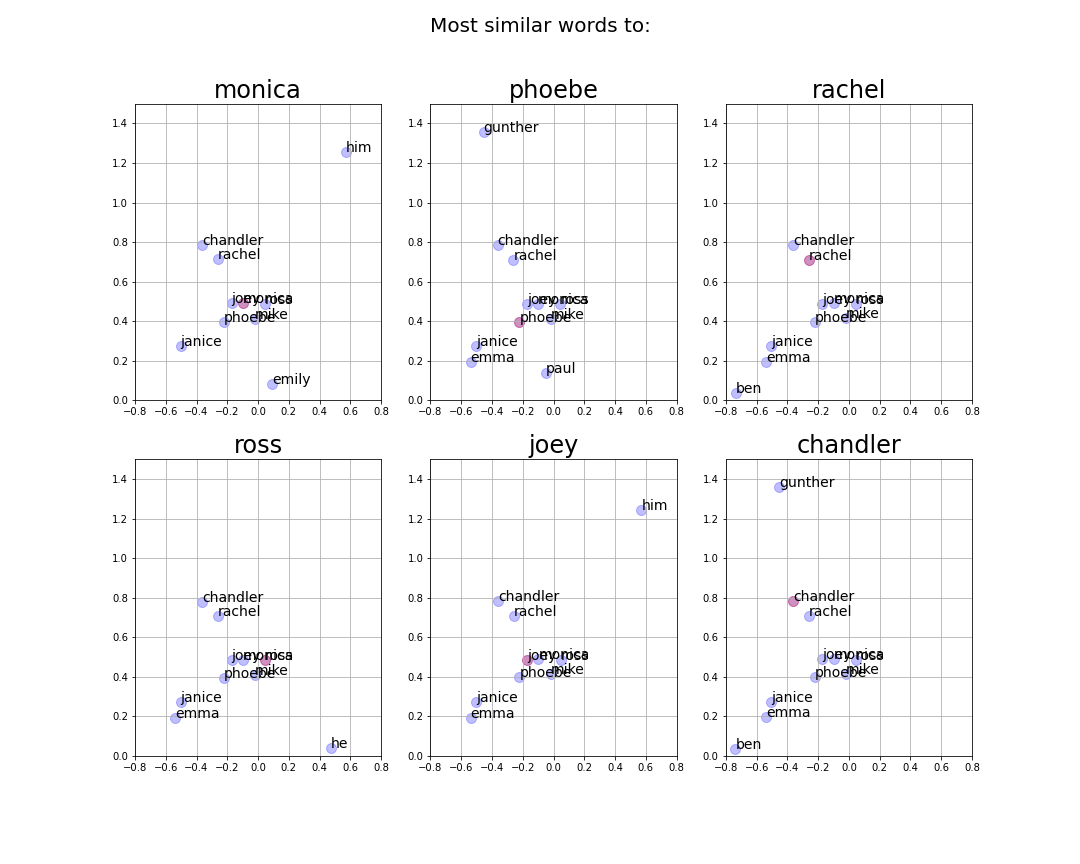
\includegraphics[width=.3\textwidth]{results/embeddings/friends_similar_15.png}\hfill
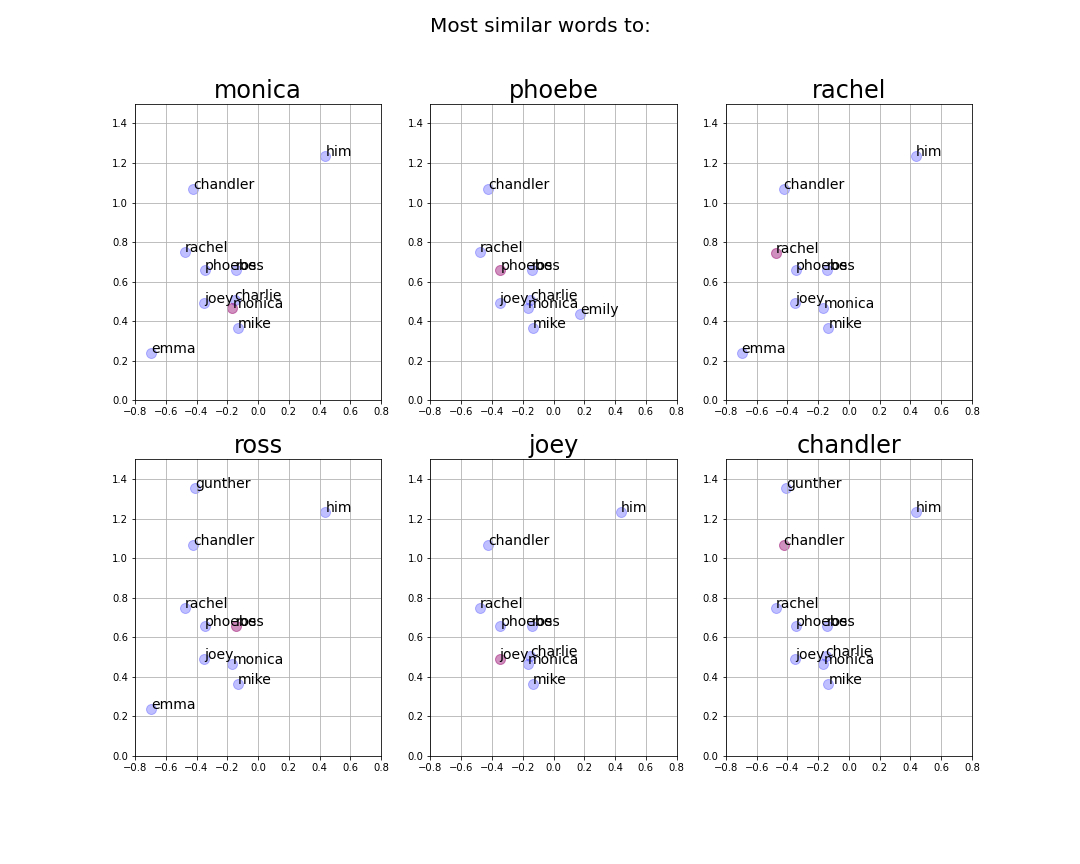
\includegraphics[width=.3\textwidth]{results/embeddings/friends_similar_75.png}\hfill
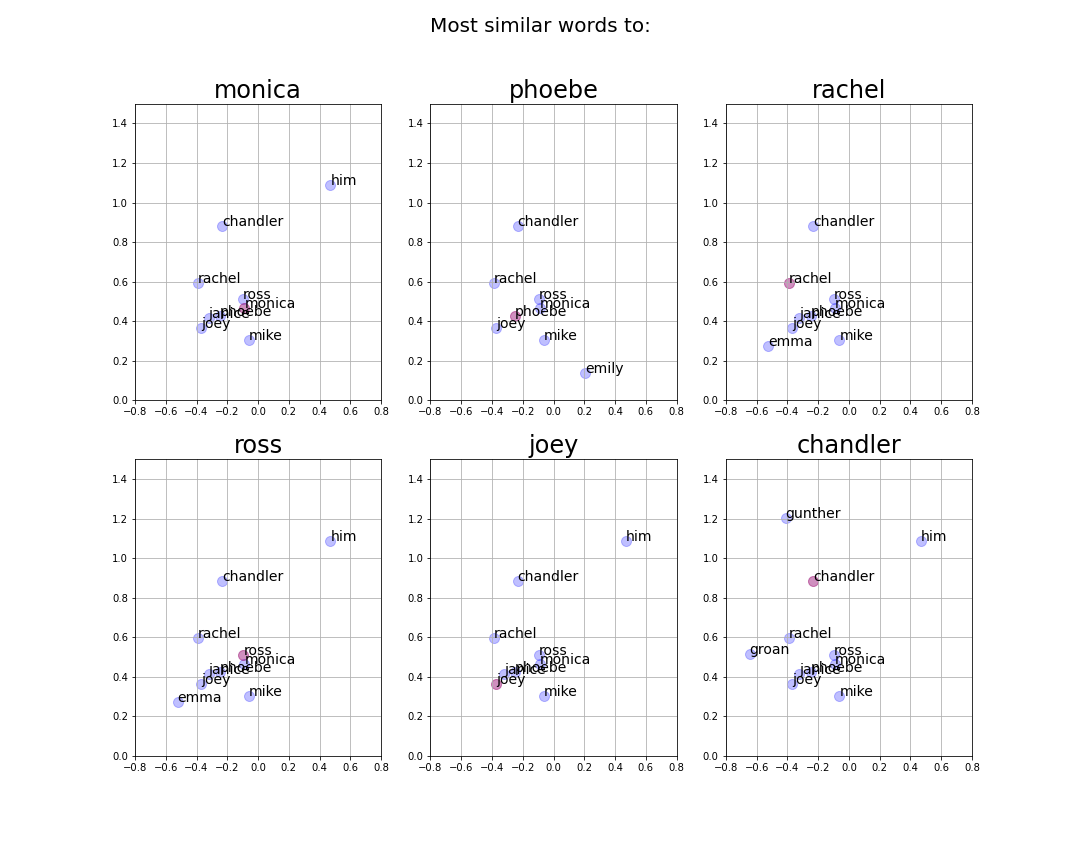
\includegraphics[width=.3\textwidth]{results/embeddings/friends_similar_150.png}
\caption{Friends main character in 2D plot with similar words for different embeddings size}
\label{fig:friends_sim_words}

\end{figure}

\subsection{Interesting Relations}
\begin{itemize}
    \item Similaridad
    
    \item Analogía 
    
    \item Coincidencia (\textit{doesn't match})
\end{itemize}

\subsubsection{Simpsons Dataset}

\begin{figure}[H]
    \centering
    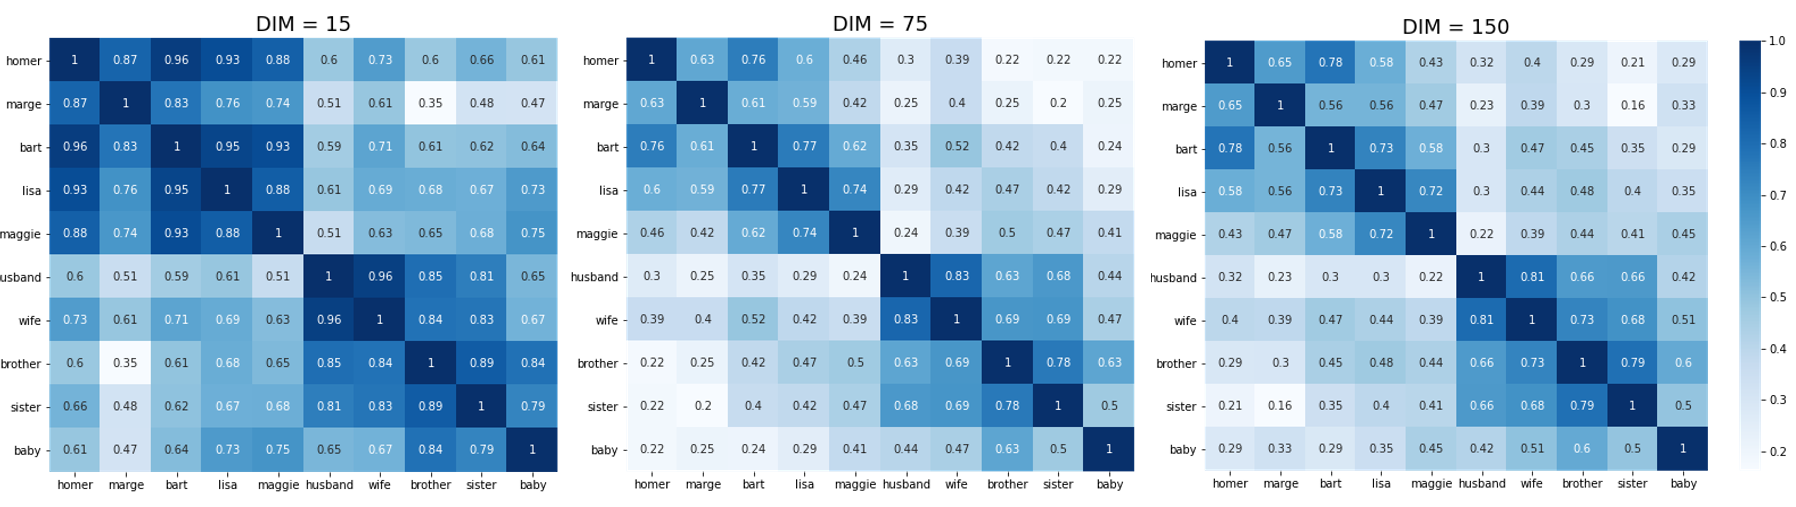
\includegraphics[width=\textwidth]{doc/images/simpsons_sim_matrix.png}
    \caption{Caption}
    \label{fig:simpsons_sim_matrix}
\end{figure}

\subsubsection{Friends Dataset}

\begin{figure}[H]
    \centering
    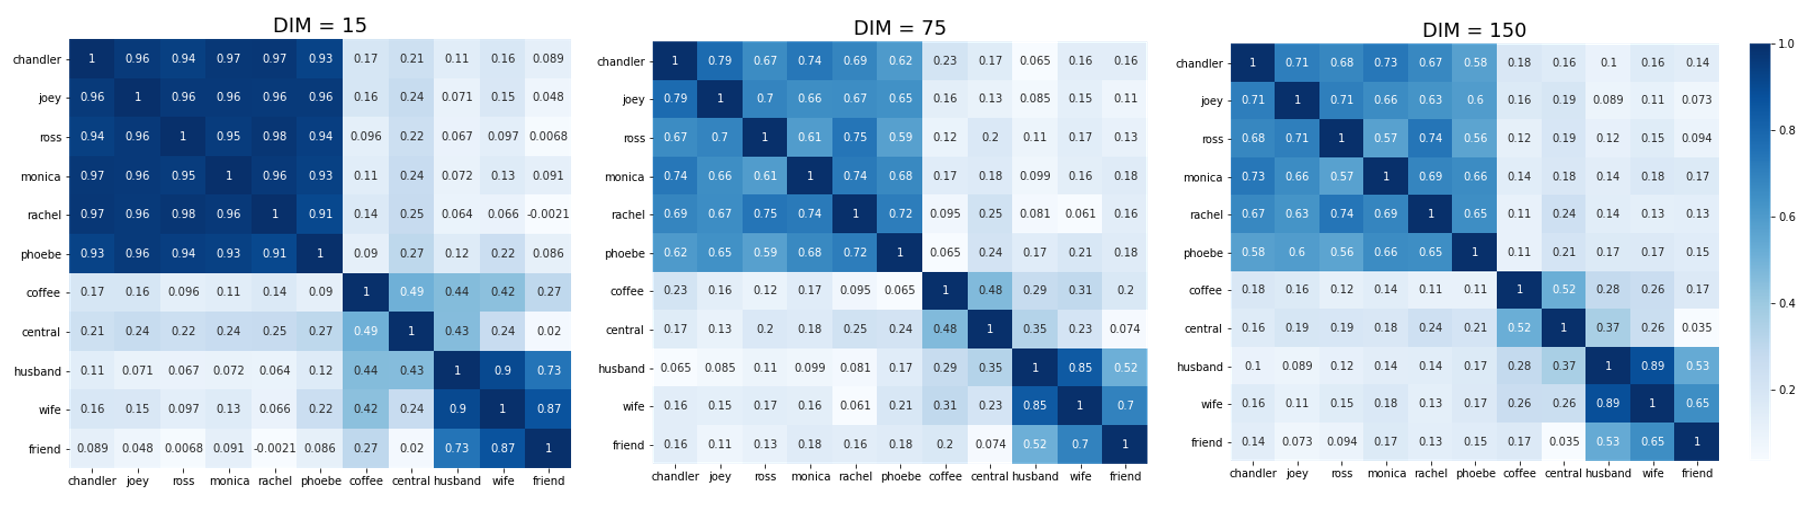
\includegraphics[width=\textwidth]{doc/images/friends_sim_matrix.png}
    \caption{Caption}
    \label{fig:friends_sim_matrix}
\end{figure}